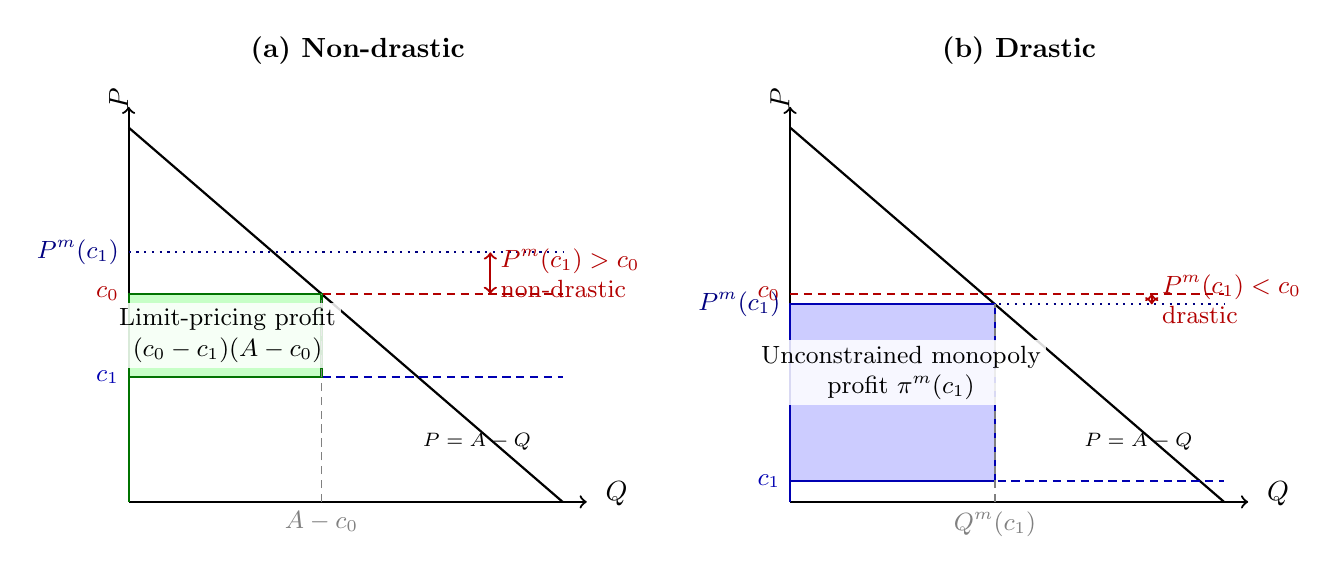
\begin{tikzpicture}
% Two-panel threshold comparison

% === Panel (a): Non-drastic ===
\begin{scope}[xshift=0cm]
\begin{axis}[
  width=7.4cm, height=6.6cm,
  xmin=0, xmax=19,
  ymin=0, ymax=19,
  axis lines=left,
  axis line style={thick, ->},
  ticks=none,
  clip=false,
  xlabel={$Q$},
  ylabel={$P$},
  xlabel style={at={(axis description cs:1.02,0.02)}, anchor=west},
  ylabel style={at={(axis description cs:0.02,1.02)}, anchor=south},
  title={\textbf{(a) Non-drastic}},
  title style={at={(0.5,1.04)}, anchor=south},
]

% Parameters: A=18, c0=10, c1=6 => P^m(c1)=12 > c0
\pgfmathsetmacro{\A}{18}
\pgfmathsetmacro{\cO}{10}
\pgfmathsetmacro{\cI}{6}
\pgfmathsetmacro{\Pm}{(\A+\cI)/2}
\pgfmathsetmacro{\Qm}{(\A-\cI)/2}
\pgfmathsetmacro{\Qpc}{\A-\cO}

% Demand and cost/price lines
\addplot[thick, domain=0:\A, samples=2, color=black] {\A - x};
\addplot[thick, densely dashed, domain=0:18, samples=2, color=red!70!black] {\cO};
\addplot[thick, densely dashed, domain=0:18, samples=2, color=blue!70!black] {\cI};
\addplot[thick, dotted, domain=0:18, samples=2, color=blue!50!black] {\Pm};

\node[anchor=east, color=red!70!black, font=\small] at (axis cs:0,\cO) {$c_0$};
\node[anchor=east, color=blue!70!black, font=\small] at (axis cs:0,\cI) {$c_1$};
\node[anchor=east, color=blue!50!black, font=\small] at (axis cs:0,\Pm) {$P^m(c_1)$};

% Non-drastic limit-pricing profit rectangle
\addplot[fill=green!22, draw=green!45!black, thick, forget plot]
  coordinates {(0,\cI) (\Qpc,\cI) (\Qpc,\cO) (0,\cO)} \closedcycle;

\addplot[densely dashed, thin, gray] coordinates {(\Qpc,0) (\Qpc,\cO)};
\node[anchor=north, gray, font=\small] at (axis cs:\Qpc,0) {$A-c_0$};

\draw[thick, <->, color=red!70!black]
  (axis cs:15,\cO) -- (axis cs:15,\Pm)
  node[midway, right, align=left, font=\small] {$P^m(c_1)>c_0$\\non-drastic};

\node[align=center, font=\small, fill=white, fill opacity=0.85, text opacity=1, inner sep=2pt]
  at (axis cs:4.1,8) {Limit-pricing profit\\$(c_0-c_1)(A-c_0)$};

\node[anchor=south west, font=\scriptsize] at (axis cs:11.8,2.0) {$P=A-Q$};
\end{axis}
\end{scope}

% === Panel (b): Drastic ===
\begin{scope}[xshift=8.4cm]
\begin{axis}[
  width=7.4cm, height=6.6cm,
  xmin=0, xmax=19,
  ymin=0, ymax=19,
  axis lines=left,
  axis line style={thick, ->},
  ticks=none,
  clip=false,
  xlabel={$Q$},
  ylabel={$P$},
  xlabel style={at={(axis description cs:1.02,0.02)}, anchor=west},
  ylabel style={at={(axis description cs:0.02,1.02)}, anchor=south},
  title={\textbf{(b) Drastic}},
  title style={at={(0.5,1.04)}, anchor=south},
]

% Parameters: A=18, c0=10, c1=1 => P^m(c1)=9.5 < c0
\pgfmathsetmacro{\A}{18}
\pgfmathsetmacro{\cO}{10}
\pgfmathsetmacro{\cI}{1}
\pgfmathsetmacro{\Pm}{(\A+\cI)/2}
\pgfmathsetmacro{\Qm}{(\A-\cI)/2}

% Demand and cost/price lines
\addplot[thick, domain=0:\A, samples=2, color=black] {\A - x};
\addplot[thick, densely dashed, domain=0:18, samples=2, color=red!70!black] {\cO};
\addplot[thick, densely dashed, domain=0:18, samples=2, color=blue!70!black] {\cI};
\addplot[thick, dotted, domain=0:18, samples=2, color=blue!50!black] {\Pm};

\node[anchor=east, color=red!70!black, font=\small] at (axis cs:0,\cO) {$c_0$};
\node[anchor=east, color=blue!70!black, font=\small] at (axis cs:0,\cI) {$c_1$};
\node[anchor=east, color=blue!50!black, font=\small] at (axis cs:0,\Pm) {$P^m(c_1)$};

% Drastic case: monopoly outcome unconstrained by fringe
\addplot[fill=blue!20, draw=blue!70!black, thick, forget plot]
  coordinates {(0,\cI) (\Qm,\cI) (\Qm,\Pm) (0,\Pm)} \closedcycle;
\addplot[densely dashed, thin, gray] coordinates {(\Qm,0) (\Qm,\Pm)};
\node[anchor=north, gray, font=\small] at (axis cs:\Qm,0) {$Q^m(c_1)$};

\draw[thick, <->, color=red!70!black]
  (axis cs:15,\Pm) -- (axis cs:15,\cO)
  node[midway, right, align=left, font=\small] {$P^m(c_1)<c_0$\\drastic};

\node[align=center, font=\small, fill=white, fill opacity=0.85, text opacity=1, inner sep=2pt]
  at (axis cs:4.6,6.2) {Unconstrained monopoly\\profit $\pi^m(c_1)$};

\node[anchor=south west, font=\scriptsize] at (axis cs:11.8,2.0) {$P=A-Q$};
\end{axis}
\end{scope}

\end{tikzpicture}
